\documentclass[]{beamer}
\usepackage[
    backend=biber,
    style=phys]{biblatex}
\usepackage{tikz}
\usepackage{graphicx}
\usepackage{braket}

\usetheme{Antibes}
\usecolortheme{beaver}
\usefonttheme[onlymath]{serif}
\addbibresource{spin_orbit_coupled_mbl_zotero_citations.bib}
%Information to be included in the title page:
\title{Localization in Spin-orbit Coupled Disordered Systems: Mid Year Report}
\author{Aditya Chincholi}
\institute{Indian Institute of Science Education and Research, Pune}

\usetikzlibrary{shapes.geometric, arrows}
\tikzstyle{startstop} = [rectangle, rounded corners, minimum width=3cm, minimum height=1cm,text centered, draw=black]
\tikzstyle{process} = [rectangle, minimum width=3cm, minimum height=1cm, text centered, text width=4.5cm, draw=black]
\tikzstyle{arrow} = [thick,->,>=stealth]



\begin{document}

\frame{\titlepage}

\begin{frame}{Table of Contents}
    \tableofcontents
\end{frame}

\section{Introduction}
\begin{frame}{Introduction}
    \begin{itemize}
        \item Disorder is almost always present in any
        material we can produce.
        \item Localization-Delocalization results in
        Metal-Insulator Transition
    \end{itemize}
\end{frame}

\begin{frame}{Introduction}
\begin{itemize}
    \item 2D Lattice
    \item Random onsite potential
    \item Fermions with spins
    \item Couple the translational motion to the spin
        of the particle through spin-orbit coupling.
\end{itemize}
\end{frame}

\begin{frame}{Why This Topic?}
    \begin{itemize}
        \item Spin adds degrees of freedom
        \item Spin-orbit coupling (SOC) adds ways to move
        that are dependent on the spin and direction of
        motion.
        \item Experimentally realizable - Cold atom
        experiments with tunable spin-orbit coupling
        \cite{orsoAndersonTransitionCold2017,
        huangExperimentalRealizationTwodimensional2016}.
    \end{itemize}
\end{frame}

\begin{frame}{But Still Why?}
    2 independent, dynamically linked densities:
    $\rho_{charge} \rightleftharpoons \rho_{spin}$
    
    Imbalance in $\rho_{c/s} \implies$ Imbalance in $\rho_{s/c}$
    \begin{itemize}
        \item Spin Patterns $\implies$ Control Particle Density.
        \item Charge Density Configuration $\implies$ Create Spin Patterns
    \end{itemize}
\end{frame}

% Add slide about the 1D spin <-> charge imbalance calc

\section{System}
\begin{frame}{What Is The System?}
    \begin{block}{Hamiltonian}
        \[
            H = \sum_{i} \epsilon_i c_i^{\dagger} c_i
            - t\sum_{<ij>} c_i^{\dagger} c_j + H_{so}
        \]
        \begin{align*}
            H_{so} = &\sum_{i}(-\alpha c_{i_{x+1}\uparrow}^{\dagger}c_{i\downarrow}
                    +\alpha c_{i_{x+1}\downarrow}^{\dagger}c_{i\uparrow}
            +\alpha c_{i_{x-1}\uparrow}^{\dagger}c_{i\downarrow}
                    -\alpha c_{i_{x-1}\downarrow}^{\dagger}c_{i\uparrow} \\
            &+ i\alpha c_{i_{y+1}\uparrow}^{\dagger}c_{i\downarrow}
                    +i\alpha c_{i_{y+1}\downarrow}^{\dagger}c_{i\uparrow}
            - i\alpha c_{i_{y-1}\uparrow}^{\dagger}c_{i\downarrow}
                    -i\alpha c_{i_{y-1}\downarrow}^{\dagger} c_{i\uparrow})
        \end{align*}
    \end{block}
    Here $\epsilon_i \in [-W/2,W/2]$ are drawn from a uniform distribution.
    $t = 1$ is the hopping strength and is usually set to unity. $\alpha$ is
    the spin-orbit coupling strength.     
\end{frame}

\begin{frame}{What Is The System?}
    \begin{tikzpicture}
        % \draw[step=1cm,gray,very thin] (-1.9,-1.9) grid (1.9,1.9);
        \node at (0,0) {$\uparrow$};
        \node at (2,0) {$\downarrow$};
        \node at (-2,0) {$\downarrow$};
        \node at (0,2) {$\downarrow$};
        \node at (0,-2) {$\downarrow$};
        \draw[thick,->] (0,0.3) -- node[anchor=west]{$i$} (0,1.7);
        \draw[thick,->] (0,-0.3) -- node[anchor=west]{$-i$} (0,-1.7);
        \draw[thick,->] (0.3,0) -- node[anchor=north]{$1$} (1.7,0);
        \draw[thick,->] (-0.3,0) -- node[anchor=north]{$-1$} (-1.7,0);
    \end{tikzpicture}
    \hfill
    \begin{tikzpicture}
        % \draw[step=1cm,gray,very thin] (-1.9,-1.9) grid (1.9,1.9);
        \node at (0,0) {$\downarrow$};
        \node at (2,0) {$\uparrow$};
        \node at (-2,0) {$\uparrow$};
        \node at (0,2) {$\uparrow$};
        \node at (0,-2) {$\uparrow$};
        \draw[thick,->] (0,0.3) -- node[anchor=west]{$i$} (0,1.7);
        \draw[thick,->] (0,-0.3) -- node[anchor=west]{$-i$} (0,-1.7);
        \draw[thick,->] (0.3,0) -- node[anchor=north]{$-1$} (1.7,0);
        \draw[thick,->] (-0.3,0) -- node[anchor=north]{$1$} (-1.7,0);
    \end{tikzpicture}    
\end{frame}

\begin{frame}{Why This System?}
    \begin{itemize}
        \item The base case of $\alpha = 0$ has been studied very well. It shows Anderson Localization \cite{abrahamsScalingTheoryLocalization1979}.
        \pause
        \item 2D is the lowest dimension where SOC makes sense.
        \pause
        \item 2D is the critical dimension for Anderson
        localization. So the effect of the SOC term will be
        very evident.
    \end{itemize}
\end{frame}

\begin{frame}{Base Case \texorpdfstring{$\alpha = 0$}{α = 0}}
    \begin{columns}
        \column{0.64\textwidth}
            \begin{itemize}
                \item $\alpha = 0 \implies$ Anderson Localization \cite{abrahamsScalingTheoryLocalization1979}
                \pause
                \item Scaling Theory\footnotemark $\implies \xi_{loc} \propto e^{a \cdot kl}$
                \item Strong Disorder $\implies kl \sim 1 \implies$ Localization observable
                \item $kl > 1$ in many cases, especially Weak Disorder
                \pause
                \item Weak Localization Correction needed in 2D
                \pause
                \item Memories of initial states retained by system \cite{chakrabortyMemoriesInitialStates2020}
            \end{itemize}    
        \column{0.33\textwidth}
            \begin{figure}[l]
                % \centering
                \includegraphics[width=\textwidth]{ahana_memories_2d_anderson_graph_crop.pdf}
                \caption{2D Anderson model (taken from \cite{chakrabortyMemoriesInitialStates2020})}
            \end{figure}    
    \end{columns}
    \footnotetext[1]{$a \approx \pi/2$, $k = 2\pi/\lambda$,
        $l$ is transport mean free path}
\end{frame}

\begin{frame}{What Will The Perturbations Do?}
    \begin{itemize}
        \item Naively, New Way to Move $\implies$ Delocalization
        \item Time-reversed Closed Paths have Opposite Spin $\implies$
        Weak Localization Correction Not Valid
    \end{itemize}
\end{frame}

% \begin{frame}{Literature Review}
%     Placeholder text
% \end{frame}

\section{Methodology}
\begin{frame}{Big Picture}
    \begin{itemize}
        \item Probe Phase Space ($W-\alpha$ plane)
        $\implies$ Calculate $\xi$ for each $(W,\alpha)$
        \item Exact Diagonalization
        \item Basis: Lattice site position basis $\times S_z$
        eigenbasis on each site 
    \end{itemize}

\end{frame}

\begin{frame}{Big Picture}
    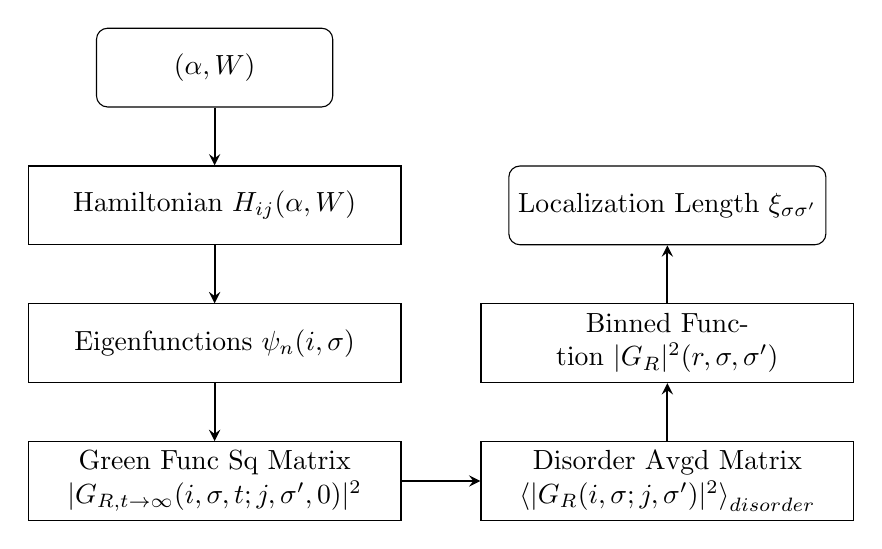
\begin{tikzpicture}[node distance=1.75cm]
        \node (start) [startstop] {$(\alpha,W)$};
        \node (ham) [process, below of=start] {Hamiltonian $H_{ij}(\alpha,W)$};
        \node (eigs) [process, below of=ham] {Eigenfunctions $\psi_n(i,\sigma)$};
        \node (gfuncsq) [process, below of=eigs] {Green Func Sq Matrix $|G_{R,t\to\infty}(i,\sigma,t;j,\sigma',0)|^2$};
        \node (disavg) [process, right of=gfuncsq, xshift=4cm] {Disorder Avgd Matrix $\braket{|G_{R}(i,\sigma;j,\sigma')|^2}_{disorder}$};
        \node (binfunc) [process, above of=disavg] {Binned Function $|G_R|^2(r,\sigma,\sigma')$};
        \node (loclen) [startstop, above of=binfunc] {Localization Length $\xi_{\sigma\sigma'}$};
        
        \draw [arrow] (start) -- (ham);
        \draw [arrow] (ham) -- (eigs);
        \draw [arrow] (eigs) -- (gfuncsq);
        \draw [arrow] (gfuncsq) -- (disavg);
        \draw [arrow] (disavg) -- (binfunc);
        \draw [arrow] (binfunc) -- (loclen);
    \end{tikzpicture}
\end{frame}


\begin{frame}{Boundary Conditions}
    \begin{itemize}
        \item Each disorder realization is not
        translationally invariant.
        \item For PBC, $\xi_{max} := ?$
        \item No good way to define $\xi$ on 2-torus if
        $\frac{\xi}{2\pi r}$ is
        non-negligible.
        \item With PBCs, the range of $r$ for our function
        $|G_R|^2(r,\sigma,\sigma')$ is halved. 
        \item Exp Decay only for large $r \implies$ We need
        points away from $r = 0$. 
        \item So we use open boundary conditions.
    \end{itemize}
\end{frame}

\begin{frame}{Kramer's Degeneracy}
    Fermionic + Time-reversal Invariant $\implies$ Kramer's Degeneracy
    $\implies$ Terms for each Degenerate Subspace
    \begin{align*}
        |G_R|^2(i,\sigma;j,\sigma') &= \sum_n |\psi_n(i,\sigma)^* \psi_n(j,\sigma')|^2\\
        &+ \sum_{E_m = E_n} \psi_n(i,\sigma)^*\psi_n(j,\sigma')\psi_m(j,\sigma')^*\psi_m(i,\sigma)
    \end{align*}
\end{frame}

\begin{frame}{Complexity}
    \begin{itemize}
        \item Summation for $|G_R|^2 \implies O(L^6)$ procedure
        \item Costliest step but no way around
        \item Decomposed as series of matrix multiplications
        \item Combine pos and spin indices $i \equiv
        (i,\sigma)$ and write eigenfunctions as a matrix:
        $\psi_k(i) = \psi_{ik}$
    \end{itemize}
\end{frame}

\begin{frame}{Complexity}
    Let $A_{ij} = |\psi_{ij}|^2$ and $B_{in} = \psi_{i,2n}^*
    \psi_{i,2n+1}$ where $i,j = 1$ to $2L^2$ and $n = 1$ to
    $L^2$. In our routines, degenerate eigenvectors come
    together.

    \begin{align*}
        \sum_{k=1}^{2L^2} |\psi_k(i)^* \psi_k(j)|^2 &= \sum_{k}|\psi_{ik}^*\psi_{jk}|^2 = \sum_k A_{ik}A_{jk} = (AA^T)_{ij}
    \end{align*}

    \begin{align*}
        &\sum_{E_m = E_k} \psi_k(i)^*\psi_k(j)\psi_m(j)^*\psi_m(i)\\
        &= \sum_{n=1}^{L^2} \psi_{i,2n}^* \psi_{j,2n} \psi_{j,2n+1}^* \psi_{i,2n+1}
        + h.c.
        = \sum_{n=1}^{L^2} B_{in} B_{jn}^* = (B B^\dagger)_{ij}
    \end{align*}    
\end{frame}

\section{Results}
\begin{frame}{Phase Space}
    \begin{figure}
        \centering
        \includegraphics[width=\textwidth]{../plots/PDFs/loc_lens_disorder_vs_coupling_heatmap_60p.pdf}
        \caption{Mean localization length for $40\times40$ over $100$ disorder realizations.}
    \end{figure}    
\end{frame}

\begin{frame}{Phase Space}
    \begin{figure}
        \centering
        \includegraphics[width=\textwidth]{../plots/PDFs/loc_lens_disorder_vs_coupling_heatmap_60p_upup.pdf}
        \caption{Up-Up localization length ($\xi_{\uparrow\uparrow}$) for $40\times40$ over $100$ disorder realizations.}
    \end{figure}    
\end{frame}

\begin{frame}{Phase Space}
    \begin{figure}
        \centering
        \includegraphics[width=\textwidth]{../plots/PDFs/loc_lens_disorder_vs_coupling_heatmap_60p_updn.pdf}
        \caption{Up-Down localization length ($\xi_{\uparrow\downarrow}$) for $40\times40$ over $100$ disorder realizations.}
    \end{figure}    
\end{frame}

\begin{frame}{Qualitative Differences}
    \begin{figure}
        \centering
        \includegraphics[width=\textwidth]{../plots/PDFs/qualitative_diffs_upup_W13_C0.3n1.0n1.5_em0.3.pdf}
        \caption{Localized phase of $|G_{\uparrow\uparrow}|^2(r)$ vs $r$ for $W = 13$ on a $40\times40$
                lattice with 100 disorder realizations.}
    \end{figure}        
\end{frame}

\begin{frame}{Qualitative Differences}
    \begin{figure}
        \centering
        \includegraphics[width=\textwidth]{../plots/PDFs/qualitative_diffs_upup_W13_C0.3n1.0n1.5_em1.0.pdf}
        \caption{Critical phase of $|G_{\uparrow\uparrow}|^2(r)$ vs $r$ for $W = 13$ on a $40\times40$
                lattice with 100 disorder realizations.}
    \end{figure}        
\end{frame}

\begin{frame}{Qualitative Differences}
    \begin{figure}
        \centering
        \includegraphics[width=\textwidth]{../plots/PDFs/qualitative_diffs_upup_W13_C0.3n1.0n1.5_em1.5.pdf}
        \caption{Delocalized phase of $|G_{\uparrow\uparrow}|^2(r)$ vs $r$ for $W = 13$ on a $40\times40$
                lattice with 100 disorder realizations.}
    \end{figure}        
\end{frame}

\begin{frame}{Qualitative Differences}
    \begin{figure}
        \centering
        \includegraphics[width=\textwidth]{../plots/PDFs/qualitative_diffs_updn_W13_C0.3n1.0n1.5_em0.3.pdf}
        \caption{Localized phase of $|G_{\uparrow\downarrow}|^2(r)$ vs $r$ for $W = 13$ on a $40\times40$
                lattice with 100 disorder realizations.}
    \end{figure}        
\end{frame}

\begin{frame}{Qualitative Differences}
    \begin{figure}
        \centering
        \includegraphics[width=\textwidth]{../plots/PDFs/qualitative_diffs_updn_W13_C0.3n1.0n1.5_em1.0.pdf}
        \caption{Critical phase of $|G_{\uparrow\downarrow}|^2(r)$ vs $r$ for $W = 13$ on a $40\times40$
                lattice with 100 disorder realizations.}
    \end{figure}        
\end{frame}

\begin{frame}{Qualitative Differences}
    \begin{figure}
        \centering
        \includegraphics[width=\textwidth]{../plots/PDFs/qualitative_diffs_updn_W13_C0.3n1.0n1.5_em1.5.pdf}
        \caption{Delocalized phase of $|G_{\uparrow\downarrow}|^2(r)$ vs $r$ for $W = 13$ on a $40\times40$
                lattice with 100 disorder realizations.}
    \end{figure}        
\end{frame}

\begin{frame}{Problems with Fitting}
    \begin{figure}
        \centering
        \includegraphics[width=\textwidth]{../plots/PDFs/fitting_diffs_W10_C0.2to0.5_em0.2.pdf}
        \caption{$|G_{\uparrow\downarrow}|^2(r)$ vs $r$ for $W = 10$ on a $40\times40$ lattice with 100 disorder realizations.}
    \end{figure}        
\end{frame}

\begin{frame}{Problems with Fitting}
    \begin{figure}
        \centering
        \includegraphics[width=\textwidth]{../plots/PDFs/fitting_diffs_W10_C0.2to0.5_em0.3.pdf}
        \caption{$|G_{\uparrow\downarrow}|^2(r)$ vs $r$ for $W = 10$ on a $40\times40$ lattice with 100 disorder realizations.}
    \end{figure}        
\end{frame}

\begin{frame}{Problems with Fitting}
    \begin{figure}
        \centering
        \includegraphics[width=\textwidth]{../plots/PDFs/fitting_diffs_W10_C0.2to0.5_em0.4.pdf}
        \caption{$|G_{\uparrow\downarrow}|^2(r)$ vs $r$ for $W = 10$ on a $40\times40$ lattice with 100 disorder realizations.}
    \end{figure}        
\end{frame}

\begin{frame}{Problems with Fitting}
    \begin{figure}
        \centering
        \includegraphics[width=\textwidth]{../plots/PDFs/fitting_diffs_W10_C0.2to0.5_em0.5.pdf}
        \caption{$|G_{\uparrow\downarrow}|^2(r)$ vs $r$ for $W = 10$ on a $40\times40$ lattice with 100 disorder realizations.}
    \end{figure}        
\end{frame}

\begin{frame}{Problems with Fitting}
    \begin{figure}
        \centering
        \includegraphics[width=\textwidth]{../plots/PDFs/fitting_diffs_W10_C0.2to0.5_upup_em0.2.pdf}
        \caption{$|G_{\uparrow\downarrow}|^2(r)$ vs $r$ for $W = 10$ on a $40\times40$ lattice with 100 disorder realizations.}
    \end{figure}        
\end{frame}

\begin{frame}{Problems with Fitting}
    \begin{figure}
        \centering
        \includegraphics[width=\textwidth]{../plots/PDFs/fitting_diffs_W10_C0.2to0.5_upup_em0.3.pdf}
        \caption{$|G_{\uparrow\uparrow}|^2(r)$ vs $r$ for $W = 10$ on a $40\times40$ lattice with 100 disorder realizations.}
    \end{figure}        
\end{frame}

\begin{frame}{Problems with Fitting}
    \begin{figure}
        \centering
        \includegraphics[width=\textwidth]{../plots/PDFs/fitting_diffs_W10_C0.2to0.5_upup_em0.4.pdf}
        \caption{$|G_{\uparrow\uparrow}|^2(r)$ vs $r$ for $W = 10$ on a $40\times40$ lattice with 100 disorder realizations.}
    \end{figure}        
\end{frame}

\begin{frame}{Problems with Fitting}
    \begin{figure}
        \centering
        \includegraphics[width=\textwidth]{../plots/PDFs/fitting_diffs_W10_C0.2to0.5_upup_em0.5.pdf}
        \caption{$|G_{\uparrow\uparrow}|^2(r)$ vs $r$ for $W = 10$ on a $40\times40$ lattice with 100 disorder realizations.}
    \end{figure}        
\end{frame}


\begin{frame}[allowframebreaks]{Bibliography}
    % \bibliographystyle{authoryear}
    \tiny{\printbibliography}
\end{frame}

\appendix
\section{Weak Localization}
\begin{frame}{Coherent Backscattering}
    The particle intensity propogator $\Phi = \braket{G^R
    G^A}$ is given by the Bethe-Salpeter equation:
    \begin{block}{Bethe-Salpeter Equation}
        \[
            \Phi = \braket{G^R G^A} = \braket{G^R}\braket{G^A}
            + \braket{G^R}\braket{G^A}U\Phi
        \]
    \end{block}
\end{frame}

\section{Green Function Squared vs Distance Fits}
\begin{frame}{Qualitative Differences}
    \begin{figure}
        \centering
        \includegraphics[width=\textwidth]{../plots/PDFs/mbl_40x40_W8_C0_TU1_TD1_N100_upup_distvsgfsq.pdf}
        \caption{$|G_{\uparrow\uparrow}|^2(r)$ vs $r$ for $W = 8.0$ $\alpha = 0$ on a $40\times40$
                lattice with 100 disorder realizations.}
    \end{figure}        
\end{frame}

\begin{frame}{Qualitative Differences}
    \begin{figure}
        \centering
        \includegraphics[width=\textwidth]{../plots/PDFs/mbl_40x40_W8_C0.1_TU1_TD1_N100_upup_distvsgfsq.pdf}
        \caption{$|G_{\uparrow\uparrow}|^2(r)$ vs $r$ for $W = 8.0$ $\alpha = 0.1$ on a $40\times40$
                lattice with 100 disorder realizations.}
    \end{figure}        
\end{frame}

\begin{frame}{Qualitative Differences}
    \begin{figure}
        \centering
        \includegraphics[width=\textwidth]{../plots/PDFs/mbl_40x40_W8_C0.2_TU1_TD1_N100_upup_distvsgfsq.pdf}
        \caption{$|G_{\uparrow\uparrow}|^2(r)$ vs $r$ for $W = 8.0$ $\alpha = 0.2$ on a $40\times40$
                lattice with 100 disorder realizations.}
    \end{figure}        
\end{frame}


\end{document}